\documentclass[%
 aip,
 jmp,%
 amsmath,amssymb,
 reprint,
]{revtex4-2}

\usepackage{graphicx}
\usepackage{dcolumn}
\usepackage{bm}
\usepackage{amsmath, amssymb, amsthm}
\usepackage{float} 

\begin{document}

\preprint{AIP/123-QED}

\title[Fundamentos de Supersimetría en Mecánica Cuántica y Factorización de Hamiltonianos]{Fundamentos de Supersimetría en Mecánica Cuántica\\ y Factorización de Hamiltonianos}

\author{Aldehil de Jesús Sánchez Hernández}
\altaffiliation[Also at ]{Ingeniería y Ciencias, ITESM}

\author{Eduardo Francisco Lugo Quintana}%
\altaffiliation[Also at ]{Ingeniería y Ciencias, ITESM}

\author{Gustavo Tellez Mireles}
\email{A01747114@tec.com}
\altaffiliation[Also at ]{Ingeniería y Ciencias, ITESM}

\author{Jorge Iván Rodríguez Reyes}
\altaffiliation[Also at ]{Ingeniería y Ciencias, ITESM}

\date{\today}

\begin{abstract}
En este trabajo se presenta un panorama general de la mecánica cuántica supersimétrica (SUSY QM) como una extensión de la mecánica cuántica convencional. Se abordan las motivaciones teóricas e históricas que dieron lugar a esta formulación y se introducen los operadores supersimétricos clave. Además, se analiza el método de factorización del Hamiltoniano y su aplicación en sistemas unidimensionales, destacando cómo, a partir de un sistema con soluciones conocidas (espectros y funciones de onda), es posible generar nuevos potenciales mediante transformaciones algebraicas. Finalmente, se discuten los principales resultados y aplicaciones de esta metodología, en particular su utilidad en el análisis espectral y la construcción de nuevos sistemas con propiedades espectrales controladas (isoespectrales).
\end{abstract}

\keywords{Supersimetría, Mecánica Cuántica, Factorización de Hamiltonianos, Superpotenciales, Potenciales periódicos, Sistemas unidimensionales.}

\maketitle
\section{Introducción}
La supersimetría en mecánica cuántica surge como una herramienta poderosa para la resolución de problemas espectrales, extendiendo el método de factorización propuesto por Schrödinger e Infeld-Hull. Este enfoque permite la obtención de nuevos potenciales a partir de un Hamiltoniano base sin alterar su espectro. Witten introdujo la supersimetría en mecánica cuántica en la década de 1980, estableciendo su relación con la teoría de campos cuánticos. Investigadores como Mielnik y Fernández han explorado la construcción de potenciales alternativos con la misma estructura espectral que el oscilador armónico.
En términos generales, la mecánica cuántica supersimétrica proporciona un marco algebraico que permite transformar sistemas cuánticos conocidos en nuevos sistemas con las mismas propiedades espectrales pero con funciones de onda modificadas. Este método ha permitido la resolución exacta de numerosos problemas en mecánica cuántica y ha encontrado aplicaciones en áreas como la física de partículas, la óptica cuántica y la teoría de solitones.
El objetivo central de este trabajo es analizar el formalismo de la mecánica cuántica supersimétrica, con énfasis en la factorización del Hamiltoniano y la construcción de superpotenciales. Se discutirán aplicaciones concretas del método, incluyendo la generación de potenciales isoespectrales y su relación con ecuaciones diferenciales no lineales. Además, se explorarán generalizaciones del método de Mielnik y su aplicación a sistemas periódicos y el oscilador armónico.

\section{Marco Teórico}
\subsection{Introducción a la mecánica cuántica supersimétrica}
La Mecánica Cuántica Supersimétrica (SUSY QM) es una versión simplificada de la supersimetría (SUSY) aplicada al ámbito de la mecánica cuántica no relativista. En lugar de enfocarse en partículas elementales y campos cuánticos, como en la SUSY de altas energías, la SUSY QM se centra en potenciales y estados ligados de sistemas cuánticos sencillos, como el oscilador armónico o el pozo de potencial.
SUSY establece la existencia de una simetría que relaciona bosones (partículas de espín entero) y fermiones (partículas de espín semientero). En SUSY QM, esta simetría se manifiesta a través de operadores, llamados supercargas, que transforman estados bosónicos en fermiónicos y viceversa.
\subsection{Definición Algebráica}
Witten, junto con otros investigadores, desarrolló la mecánica cuántica supersimétrica como un "laboratorio" para explorar las ideas de la supersimetría en un contexto más simple. SUSY QM introduce operadores supercargas, $Q$ y $Q^{\dagger}$, que satisfacen un álgebra particular que involucra al Hamiltoniano $H$:
\begin{equation}
Q_1 = \frac{Q^+ + Q^-}{\sqrt{2}}, \quad
Q_2 = \frac{Q^+ - Q^-}{i\sqrt{2}}, \quad
\{Q, Q^{\dagger}\} = H, \quad Q^2 = (Q^{\dagger})^2 = 0.
\end{equation}
Estos operadores son matrices porque en el contexto de la mecánica cuántica supersimétrica, la supersimetría se representa como una simetría que mezcla dos sectores diferentes del sistema: el bosónico y el fermiónico. Estos sectores se modelan mediante una representación matricial, donde cada bloque representa la acción del operador en uno de los sectores.
La razón por la cual se definen de esta manera es que, en el marco de la supersimetría, se quería que estos operadores conserven la estructura algebraica que permite la descomposición del Hamiltoniano supersimétrico.
\begin{equation}
Q^+ = \begin{pmatrix} 0 & B_k^+ \\ 0 & 0 \end{pmatrix}, \quad Q^- = \begin{pmatrix} 0 & 0 \\ B_k^- & 0 \end{pmatrix}.
\end{equation}
El Hamiltoniano supersimétrico toma la forma:
\begin{equation}
H_{ss} = \{Q^-, Q^+\} = \begin{pmatrix} B_k^+ B_k^- & 0 \\ 0 & B_k^- B_k^+ \end{pmatrix}.
\end{equation}
\subsection{Entrelazamiento operatorial y SUSY QM}
El método de entrelazamiento operatorial, desarrollado posteriormente, proporciona una herramienta poderosa para construir sistemas supersimétricos. Este método se basa en la idea de entrelazar dos Hamiltonianos \( H_0 \) y \( H_1 \) a través de un operador \( A \):
\begin{equation}
H_1 = A H_0 A^{-1}
\end{equation}
En el contexto de SUSY QM, el operador de entrelazamiento A se relaciona directamente con los operadores supercargas Q y Q†. Específicamente, A puede construirse a partir de una combinación lineal de estos operadores. Esto permite generar pares de Hamiltonianos supersimétricos de manera sistemática, facilitando el estudio de sus propiedades y la exploración de la ruptura de la supersimetría.
\subsection{Superpotencial y la ecuación de Riccati}
El método de entrelazamiento operatorial está íntimamente ligado al concepto de superpotencial \( W(x) \) en SUSY QM. Este superpotencial es una función que determina completamente los Hamiltonianos \( H_0 \) y \( H_1 \) del sistema supersimétrico. 
El superpotencial \( W(x) \) encapsula la información esencial que define la estructura del sistema supersimétrico, y a partir de él se construyen los Hamiltonianos \( H_0 \) y \( H_1 \).
Dado un Hamiltoniano base unidimensional:
\begin{equation}
H_0 = -\frac{d^2}{dx^2} + V_0(x),
\end{equation}
Donde se tiene un H1 que esta anclado a lo que se proponga para H0 de la siguiente manera:
\begin{equation}
H_0 = -\frac{d^2}{dx^2} + V_0(x),
h_1 = -\frac{d^2}{dx^2} + W^2(x) + W'(x)
\end{equation}
Esto debido a que tras la factorización del Hamiltoniano obtenemos la ecuación fundamental: 
\begin{equation}
V_0(x) = W^2(x) + W'(x).
\end{equation}
La cual es una ecuación de Riccatti, que en su forma general es: 
\begin{equation}
y'(x) + y^2(x) = f(x)
\end{equation}
Si identificamos
\begin{equation}
y(x) = W(x) y f(x) = V_0(x)
\end{equation}
, la ecuación de transformación del potencial se reescribe como
\begin{equation}
W'(x) + W^2(x) = V_0(x).
\end{equation}
En la mecánica cuántica supersimétrica estándar (SUSY QM de primer orden), se usa una única función semilla \( \psi_1(x) \) (que es una solución de la ecuación de Schrödinger para \( H_0 \)), y el nuevo potencial se obtiene a partir del superpotencial:
\begin{equation}
W(x) = \frac{\psi_0'(x)}{\psi_0(x)}.
\end{equation}
El potencial transformado resulta ser:
\begin{equation}
V_1(x) = V_0(x) - 2W'(x)
\end{equation}
En lugar de usar solo una función semilla, ahora usamos un conjunto de k soluciones linealmente independientes de la ecuación de Schrödinger para \( H_0 \):
\begin{equation}
H_0 \psi_i = E_i \psi_i, \quad i = 1, 2, \dots, k.
\end{equation}
A partir de estas funciones, se construye el wronskiano:
\begin{equation}
W(\psi_1, \psi_2, \dots, \psi_k) =
\begin{vmatrix}
\psi_1 & \psi_2 & \dots & \psi_k \\
\psi_1' & \psi_2' & \dots & \psi_k' \\
\vdots & \vdots & \ddots & \vdots \\
\psi_1^{(k-1)} & \psi_2^{(k-1)} & \dots & \psi_k^{(k-1)}
\end{vmatrix}
\end{equation}
El nuevo potencial transformado se obtiene mediante:
\begin{equation}
V_k(x) = V_0(x) - 2 \frac{d^2}{dx^2} \ln W(\psi_1, \psi_2, \dots, \psi_k)
\end{equation}
La cual cumple con el álgebra propuesto por Witten tiempo atrás.

\section{Desarrollo teórico}
En esta sección, profundizamos en el método de Darboux para la eliminación de estados del oscilador armónico, utilizando el formalismo de la mecánica cuántica supersimétrica y la factorización de Hamiltonianos. El objetivo es modificar el espectro del oscilador armónico, eliminando k estados consecutivos a partir del n-ésimo nivel.
Teniendo en cuenta el Hamiltoniano del oscilador armónico cuántico:
\begin{equation}
H_0 = -\frac{\hbar^2}{2m} \frac{d^2}{dx^2} + \frac{1}{2} m \omega^2 x^2
\end{equation}
Para simplificar, utilizaremos unidades adimensionales donde \( \hbar = m = \omega = 1 \). Así, el Hamiltoniano se reduce a:
\begin{equation}
H_0 = -\frac{1}{2} \frac{d^2}{dx^2} + \frac{1}{2} x^2
\end{equation}
De esta forma, la solución de la función de onda para la ecuación Schrödinger, del oscilador armónico, puede ser descrita en términos de polinomios de Hermite de la siguiente manera:
\begin{equation}
\psi_n(x) = H_n(x) e^{-\frac{x^2}{2}}
\end{equation}
A partir del Hamiltoniano \( H_0 \), se puede conocer el potencial base \( V_0 \):
\begin{equation}
V_0=\frac{1}{2} x^2
\end{equation}
\begin{figure}[H]
    \centering
    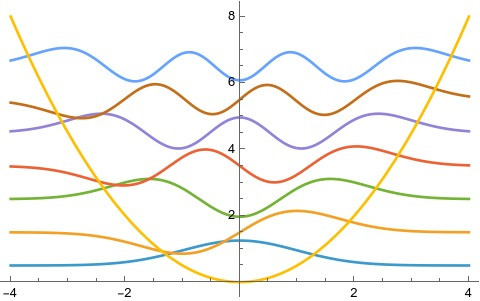
\includegraphics[width=0.6\textwidth]{QuantumHarmonicOscillator.jpeg}
    \caption{Gráfica de los estados del oscilador armónico y su potencial.}
    \label{fig:modified_oscillator}
\end{figure}
A partir del potencial \( V_0 \) podemos encontrar un nuevo potencial aplicando la siguiente ecuación (transformada de Darboux):
\begin{equation}
V_k(x) = V_0(x) - 2 \frac{d^2}{dx^2} \ln(W(\psi_1, \psi_2, ..., \psi_k))
\end{equation}
Donde \( \psi_1, \psi_2, \dots, \psi_k \) son los \( k \) estados consecutivos que deseamos eliminar (funciones semillas).
Para ejemplificar, utilizamos \( \psi_2 \) y \( \psi_3 \) como nuestras funciones semillas:
\begin{equation}
V_k(x) = V_0(x) - 2 \frac{d^2}{dx^2} \ln(W(\psi_2, \psi_3))
\end{equation}
\begin{figure}[H]
    \centering
    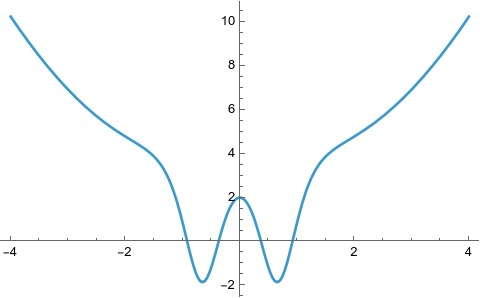
\includegraphics[width=0.6\textwidth]{QuantumHarmonicOscillator_blue_2_2.jpeg}
    \caption{Gráfica del potencial modificado del oscilador armónico con nb=2 y k=2.}
    \label{fig:modified_oscillator}
\end{figure}
También generamos el operador \( B_k \):
\begin{equation}
B_k = \frac{W(\psi_1, \psi_2, \dots, \psi_k, \psi_n)}{W(\psi_1, \psi_2, \dots, \psi_k)}
\end{equation}
Al aplicar el operador \( B_k \) a cada uno de los estados del oscilador, los estados que definimos como nuestras funciones semillas se vuelven 0:
\begin{figure}[H]
    \centering
    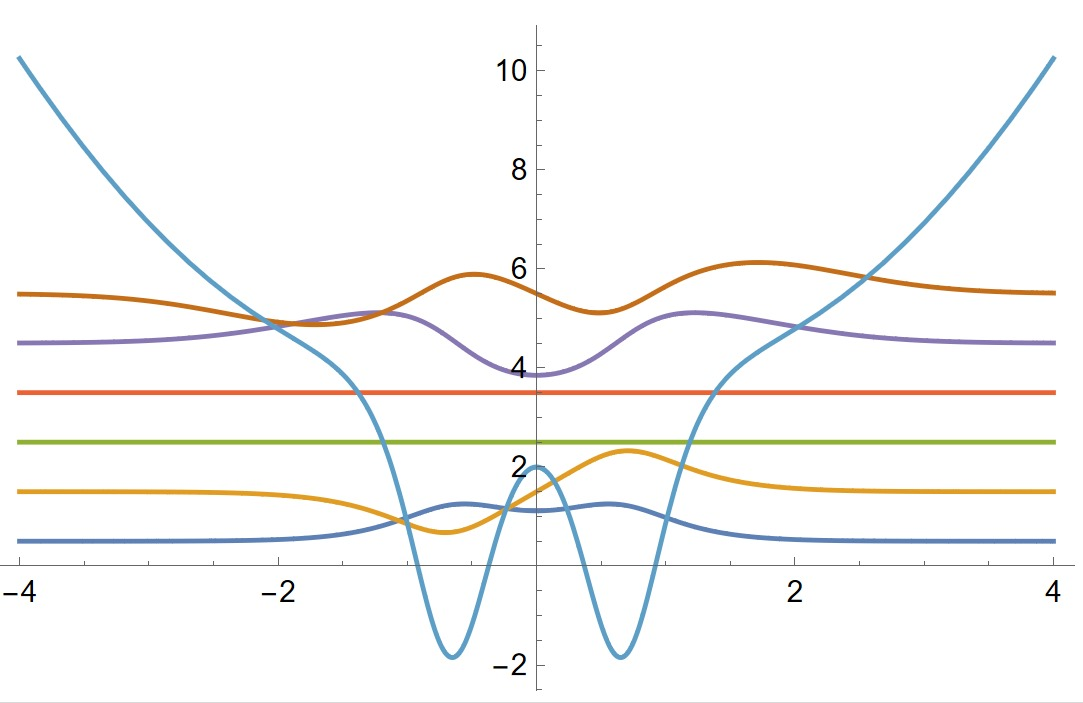
\includegraphics[width=0.6\textwidth]{QuantumHarmonicOscillator_2_3.jpeg}
    \caption{Gráfica con los estados eliminados del oscilador armónico y el potencial modificado.}
    \label{fig:modified_oscillator}
\end{figure}

\section{Discusión}
Partiendo de las consideraciones anteriores, cuando se eligen semillas consecutivas 
\( \psi_n, \psi_{n+1}, \dots, \psi_{n+k-1} \), la forma en que sus ceros reales se “superponen” depende del valor de \( k \). 

Concisamente, para \( k \) par, los ceros de algunas funciones se compensan con la estructura de otras y generan un Wronskiano que no se anula en el eje real, evitando la aparición de ceros comunes. 

Con \( k \) impar, se elimina la compensación mencionada, por lo que el Wronskiano presenta puntos donde se anula, produciendo singularidades (picos) en \( V_k(x) \). 

Para ilustrar estas singularidades, cuando se declara \( k = 3 \) (tres funciones semillas), se obtiene la siguiente gráfica:

\begin{figure}[H]
    \centering
    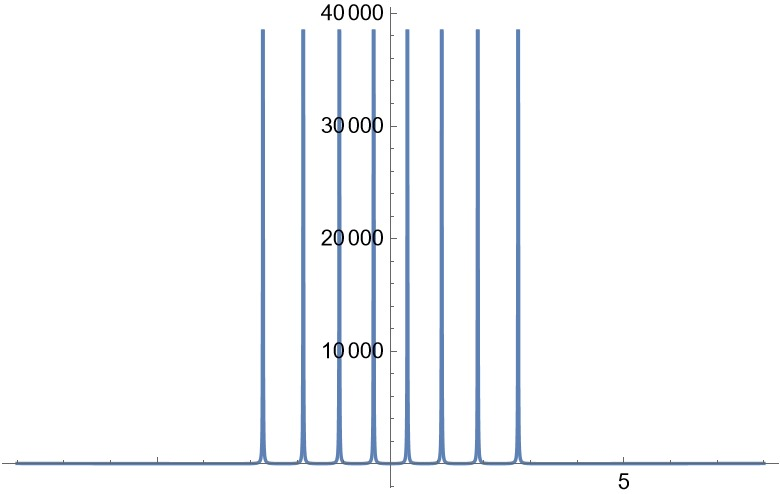
\includegraphics[width=0.6\textwidth]{QHO_Odd.jpeg}
    \caption{Potencial Modificado con k impar.}
    \label{fig:modified_oscillator}
\end{figure}
Podemos visualizar los picos que representan las posiciones donde el Wronksiano se anula y el nuevo potencial se hace infinito, o sea, cuando:
\begin{equation}
W(\psi_8, \psi_9, \psi_{10})(x)=0
\end{equation}
Puesto que considerando nuevamente la transformada de Darboux para el oscilador armónico:
\begin{equation}
V_k(x) = \frac{1}{2} x^2 - 2 \frac{d^2}{dx^2} \ln \left( W(\psi_8, \psi_9, \psi_{10}) \right),
\end{equation}
en esos puntos, \( \ln(W(\dots)) \) diverge y la segunda derivada se hace infinita.

\section{Conclusiones}
Este trabajo ha demostrado cómo la mecánica cuántica supersimétrica (SUSY QM) y la factorización de Hamiltonianos permiten modificar y controlar la estructura espectral de sistemas cuánticos, destacando su aplicación en la generación de potenciales isoespectrales y la eliminación de estados en el oscilador armónico. La conexión con la ecuación de Riccati y el uso del wronskiano en transformaciones de Darboux han sido clave para comprender la construcción de nuevos potenciales, identificando cómo la elección de funciones semilla puede generar o evitar singularidades en el sistema. A futuro, este enfoque puede extenderse a sistemas en más dimensiones, aplicarse en la teoría de bandas en materiales cuánticos, explorarse en el contexto de ecuaciones no lineales y analizarse en experimentos con trampas de iones o condensados de Bose-Einstein. En definitiva, el formalismo de SUSY QM se presenta como una herramienta versátil con un gran potencial de aplicación en diversas áreas de la física teórica y aplicada.

\nocite{*}
\maketitle
\section{Referencias}
\bibliography{aipsamp}% Produces the bibliography via BibTeX.

\section{Agradecimientos}

Queremos expresar nuestro más sincero agradecimiento a nuestros profesores, quienes han sido fundamentales en nuestra formación académica y en el desarrollo de este trabajo.

A la Dra. Zurika Iveth Blanco García, por su paciencia y dedicación en la enseñanza del álgebra cuántica y Mathematica.

Al Dr. Mario Iván Estrada Delgado, por proporcionarnos artículos y recursos de gran utilidad, así como por plantearnos ejercicios desafiantes que fortalecieron nuestras habilidades en la resolución de problemas avanzados.

Al Dr. Fernando Olivar Romero, por sentar las bases de nuestra comprensión en mecánica cuántica.

Asimismo, agradecemos el uso de herramientas de inteligencia artificial, las cuales nos asistieron en la redacción y mejora de la escritura de fórmulas en este trabajo.

\end{document}
